\subsection{Results and discussion}\label{sec:m3:results}
    
    ~\cref{fig:m3:potentials} shows the metric perturbation potentials $\Phi$ and $\Psi$ as functions of time $x$ for the $k$-modes under investigation. The time of matter-radiation equality and recombination is marked in the plot as black dash-dotted and dashed lines respectively. Let's first consider the top panel, showing only $\Phi$. At early times, it seems to be constant across all $k$-modes. \footnote{When referring to ``all $k$-modes'' it is implicit that we only mean the three modes considered here, but the qualitative discussions should be valid across all $k$-modes.} This is expected since at early times, the horizon is small and most modes are larger than this. Thus, they will be unaffected by causal physics and stay constant at their initial value. As time proceeds, the smaller $k$-modes will be surpassed by the horizon and are suddenly subjected to causal physics. We see from the top panel that if this happens in the radiation dominated regime (before radiation-matter equality), the potential will decline as $e^{-2x}$. This can be seen from ~\cref{eq:m3:theory:phi_perturbation} 
    \begin{figure}
        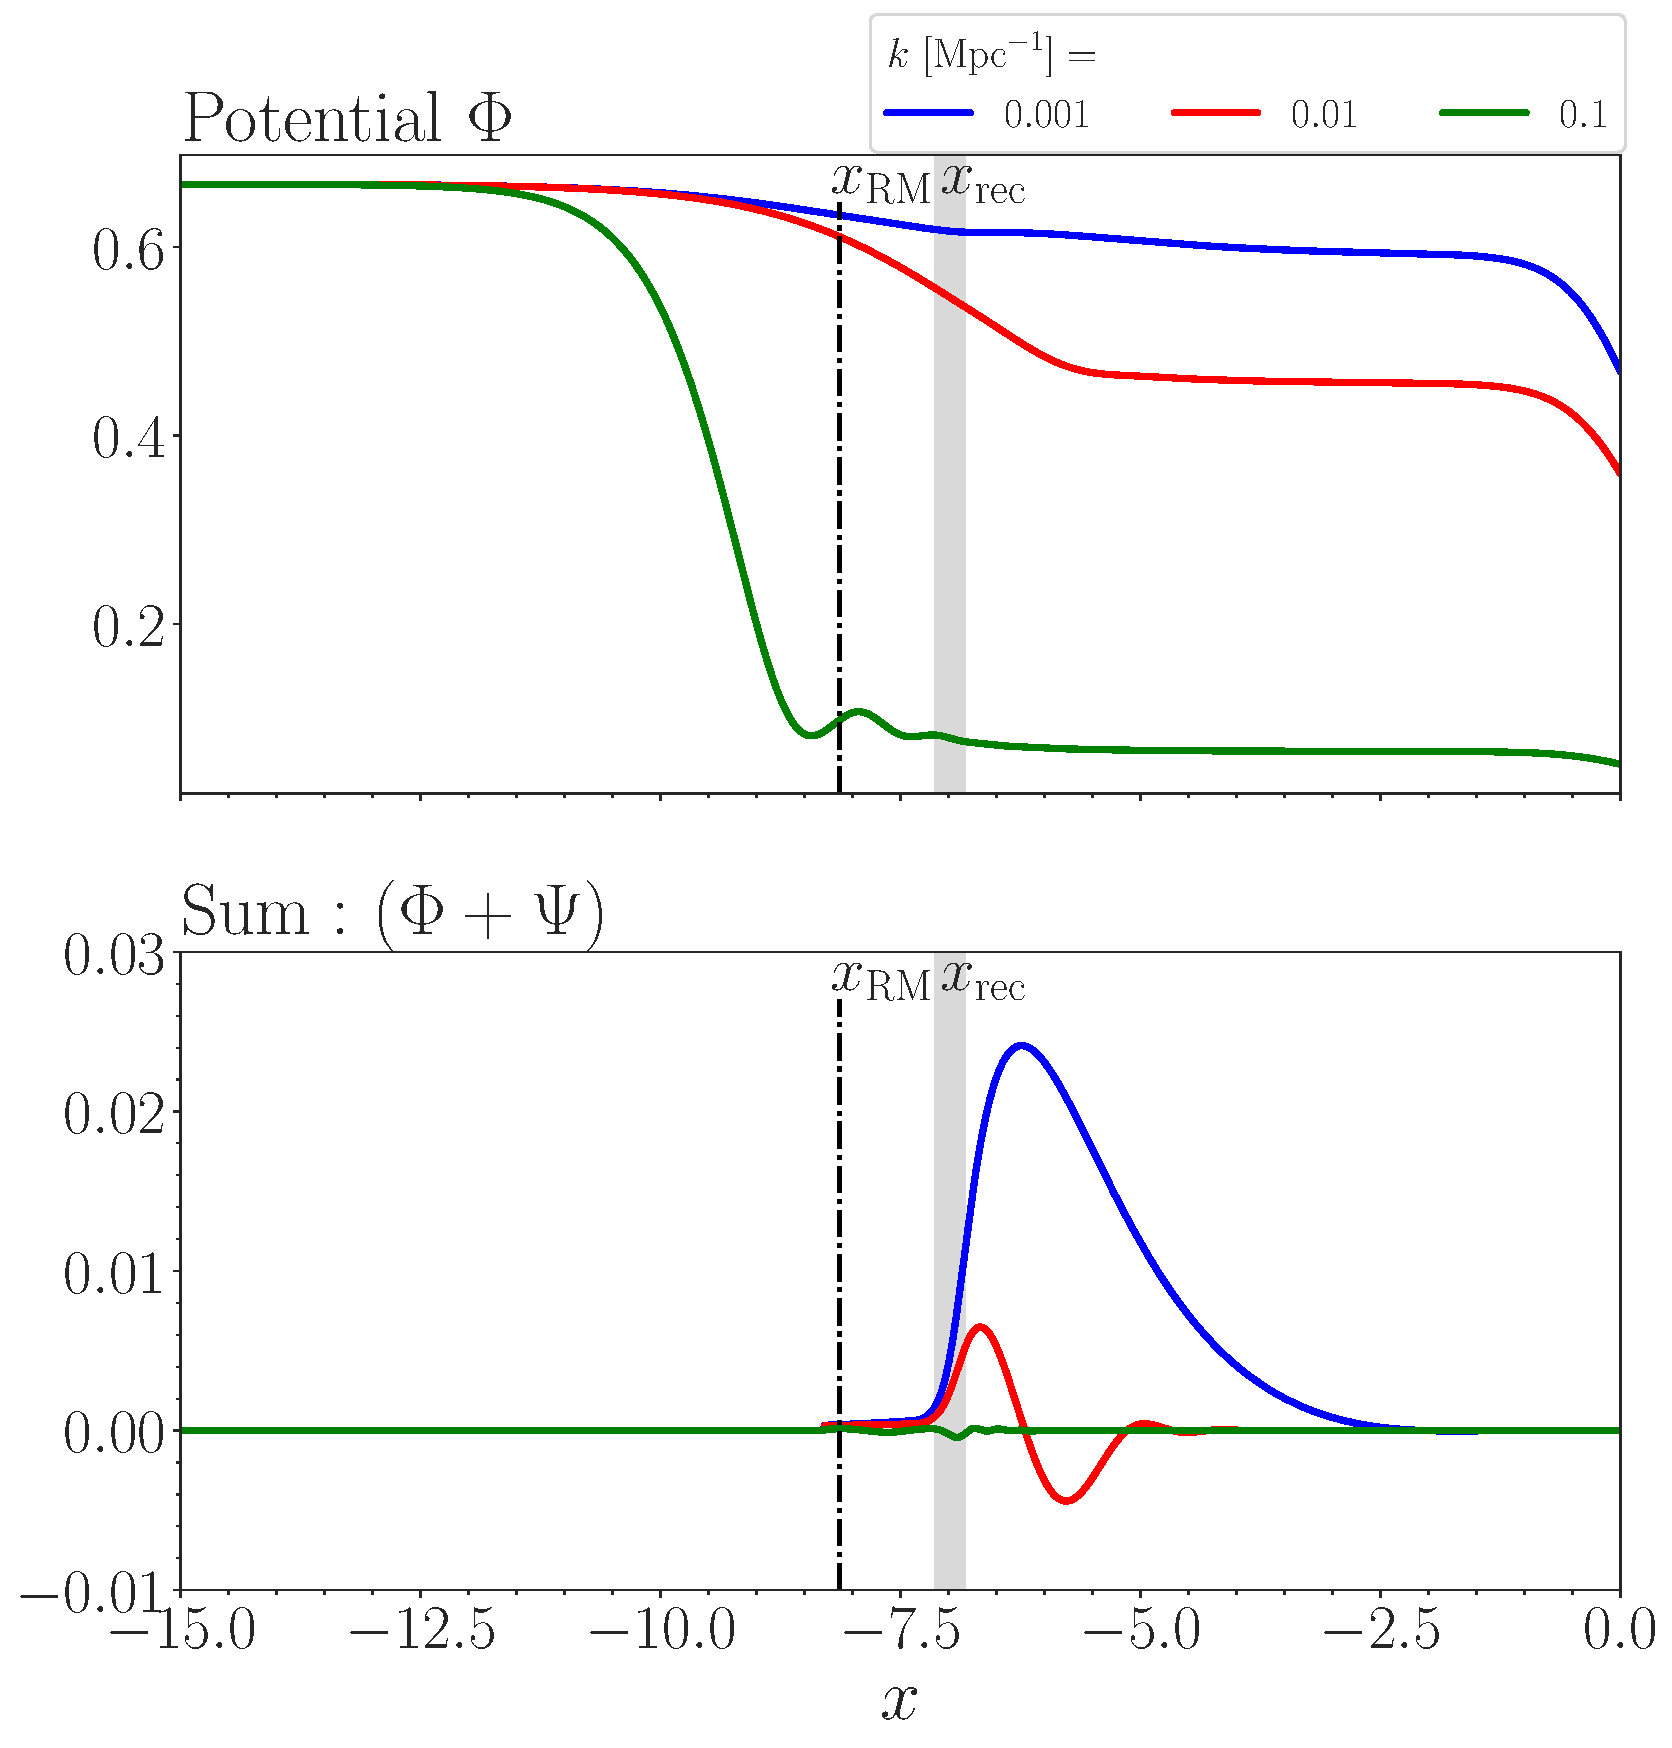
\includegraphics[width=\linewidth]{potentials.pdf}
        \caption{The metric perturbation potentials, $\Psi$ representing the Newtonian potential, and $\Phi$ representing the spatial curvature perturbations. Both panels show the evolution as function of the time $x$, for the three different $k$-modes outlined in ~\cref{sec:m3:methods}. The top panel shows $\Phi$ alone, while the bottom shows the sum of the two. The dashed black line is the time of recombination as found in ~\cref{sec:m2}, and the dash-dotted black line is the time of radiation-matter equality as found in ~\cref{sec:m1}.}
        \label{fig:m3:potentials}
    \end{figure}

    \begin{figure}
        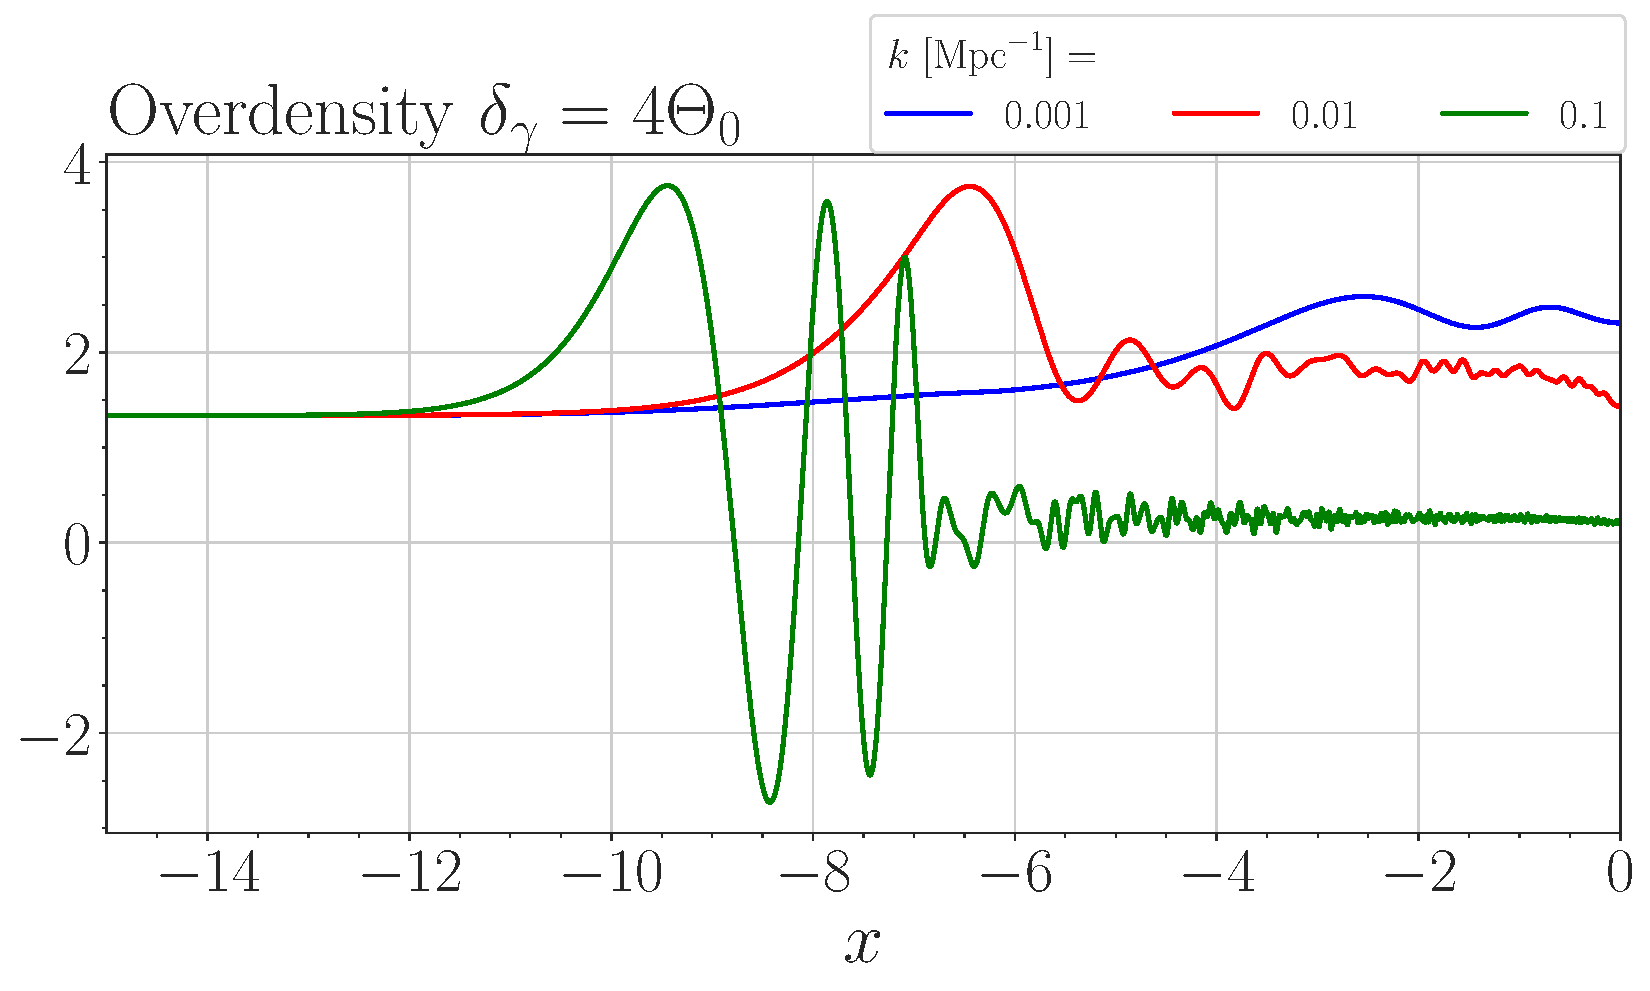
\includegraphics[width=\linewidth]{monopole.pdf}
        \caption{Monopole term The dashed black line is the time of recombination as found in ~\cref{sec:m2}, and the dash-dotted black line is the time of radiation-matter equality as found in ~\cref{sec:m1}.}
        \label{fig:m3:monopole}
    \end{figure}

    \begin{figure}
        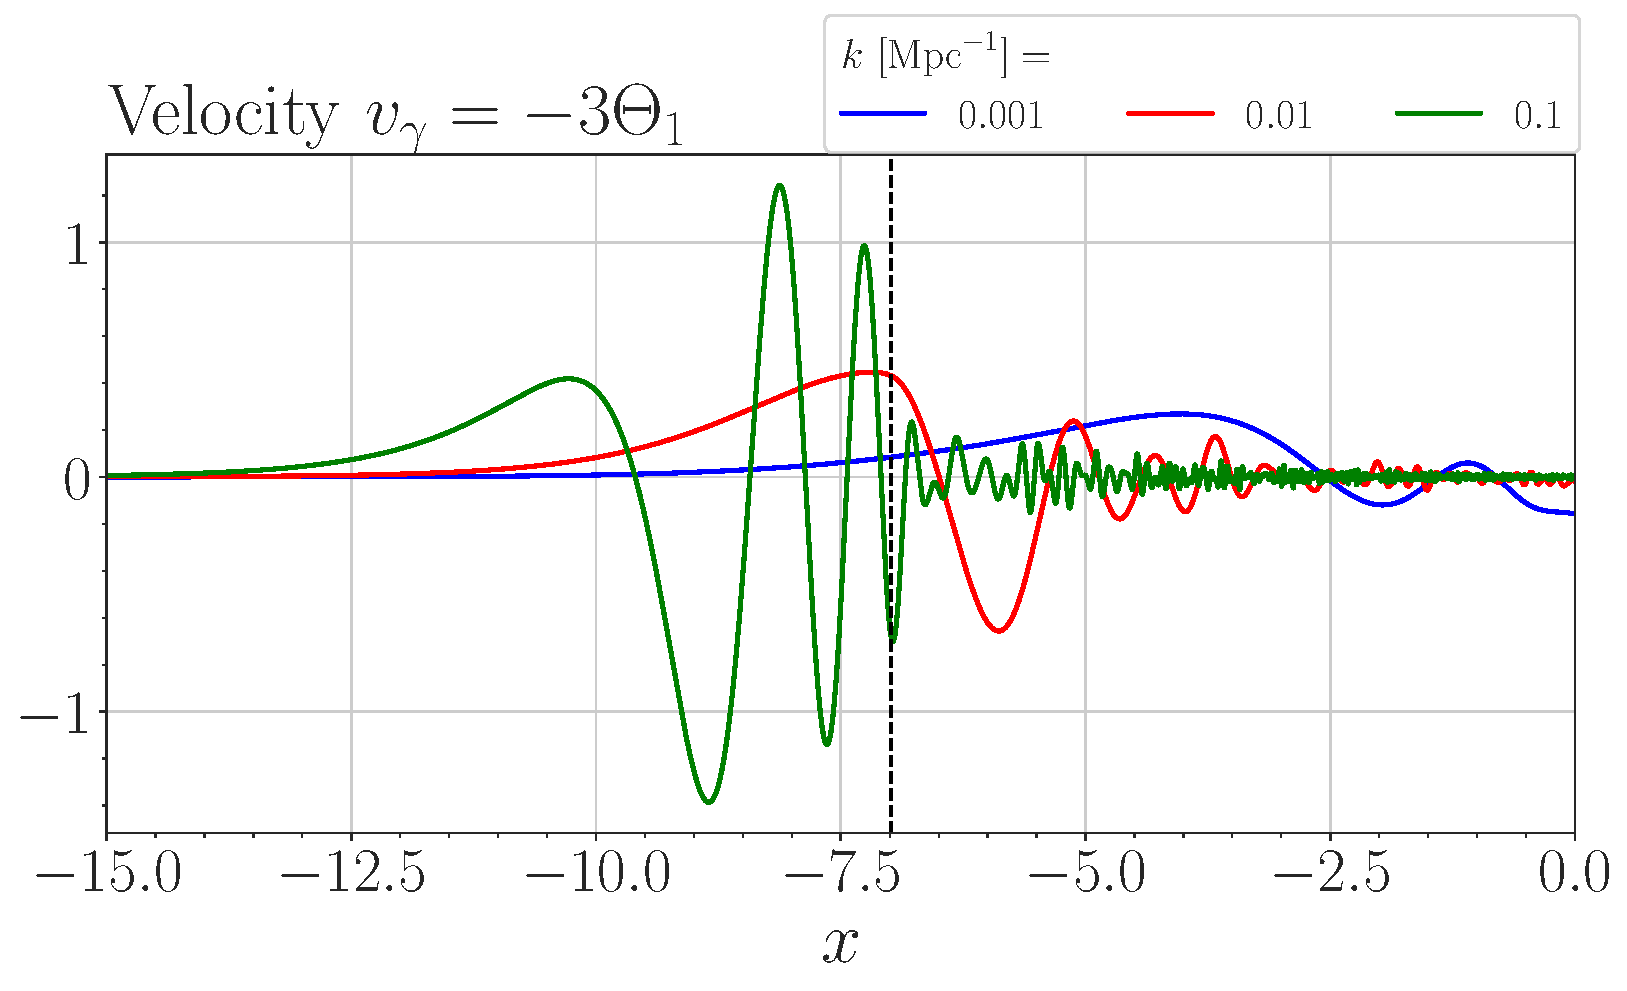
\includegraphics[width=\linewidth]{dipole.pdf}
        \caption{Dipole term The dashed black line is the time of recombination as found in ~\cref{sec:m2}, and the dash-dotted black line is the time of radiation-matter equality as found in ~\cref{sec:m1}.}
        \label{fig:m3:dipole}
    \end{figure}

    \begin{figure}
        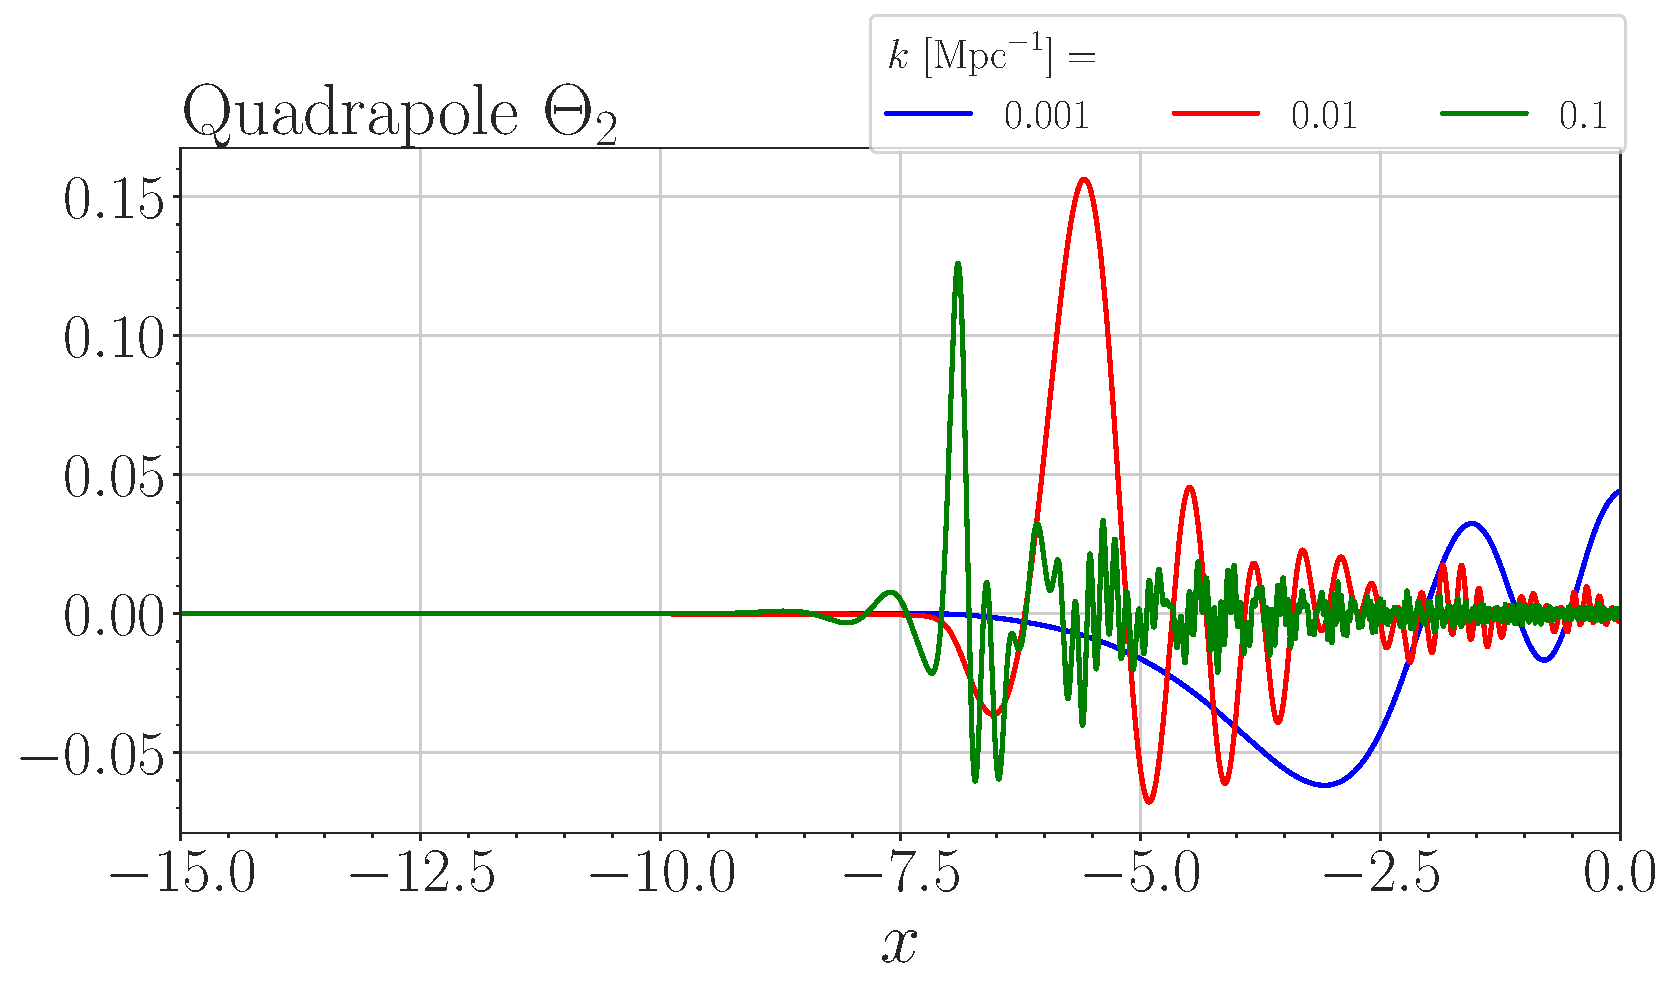
\includegraphics[width=\linewidth]{quadrapole.pdf}
        \caption{Quadrapole term The dashed black line is the time of recombination as found in ~\cref{sec:m2}, and the dash-dotted black line is the time of radiation-matter equality as found in ~\cref{sec:m1}.}
        \label{fig:m3:quadrapole}
    \end{figure}

    \begin{figure}
        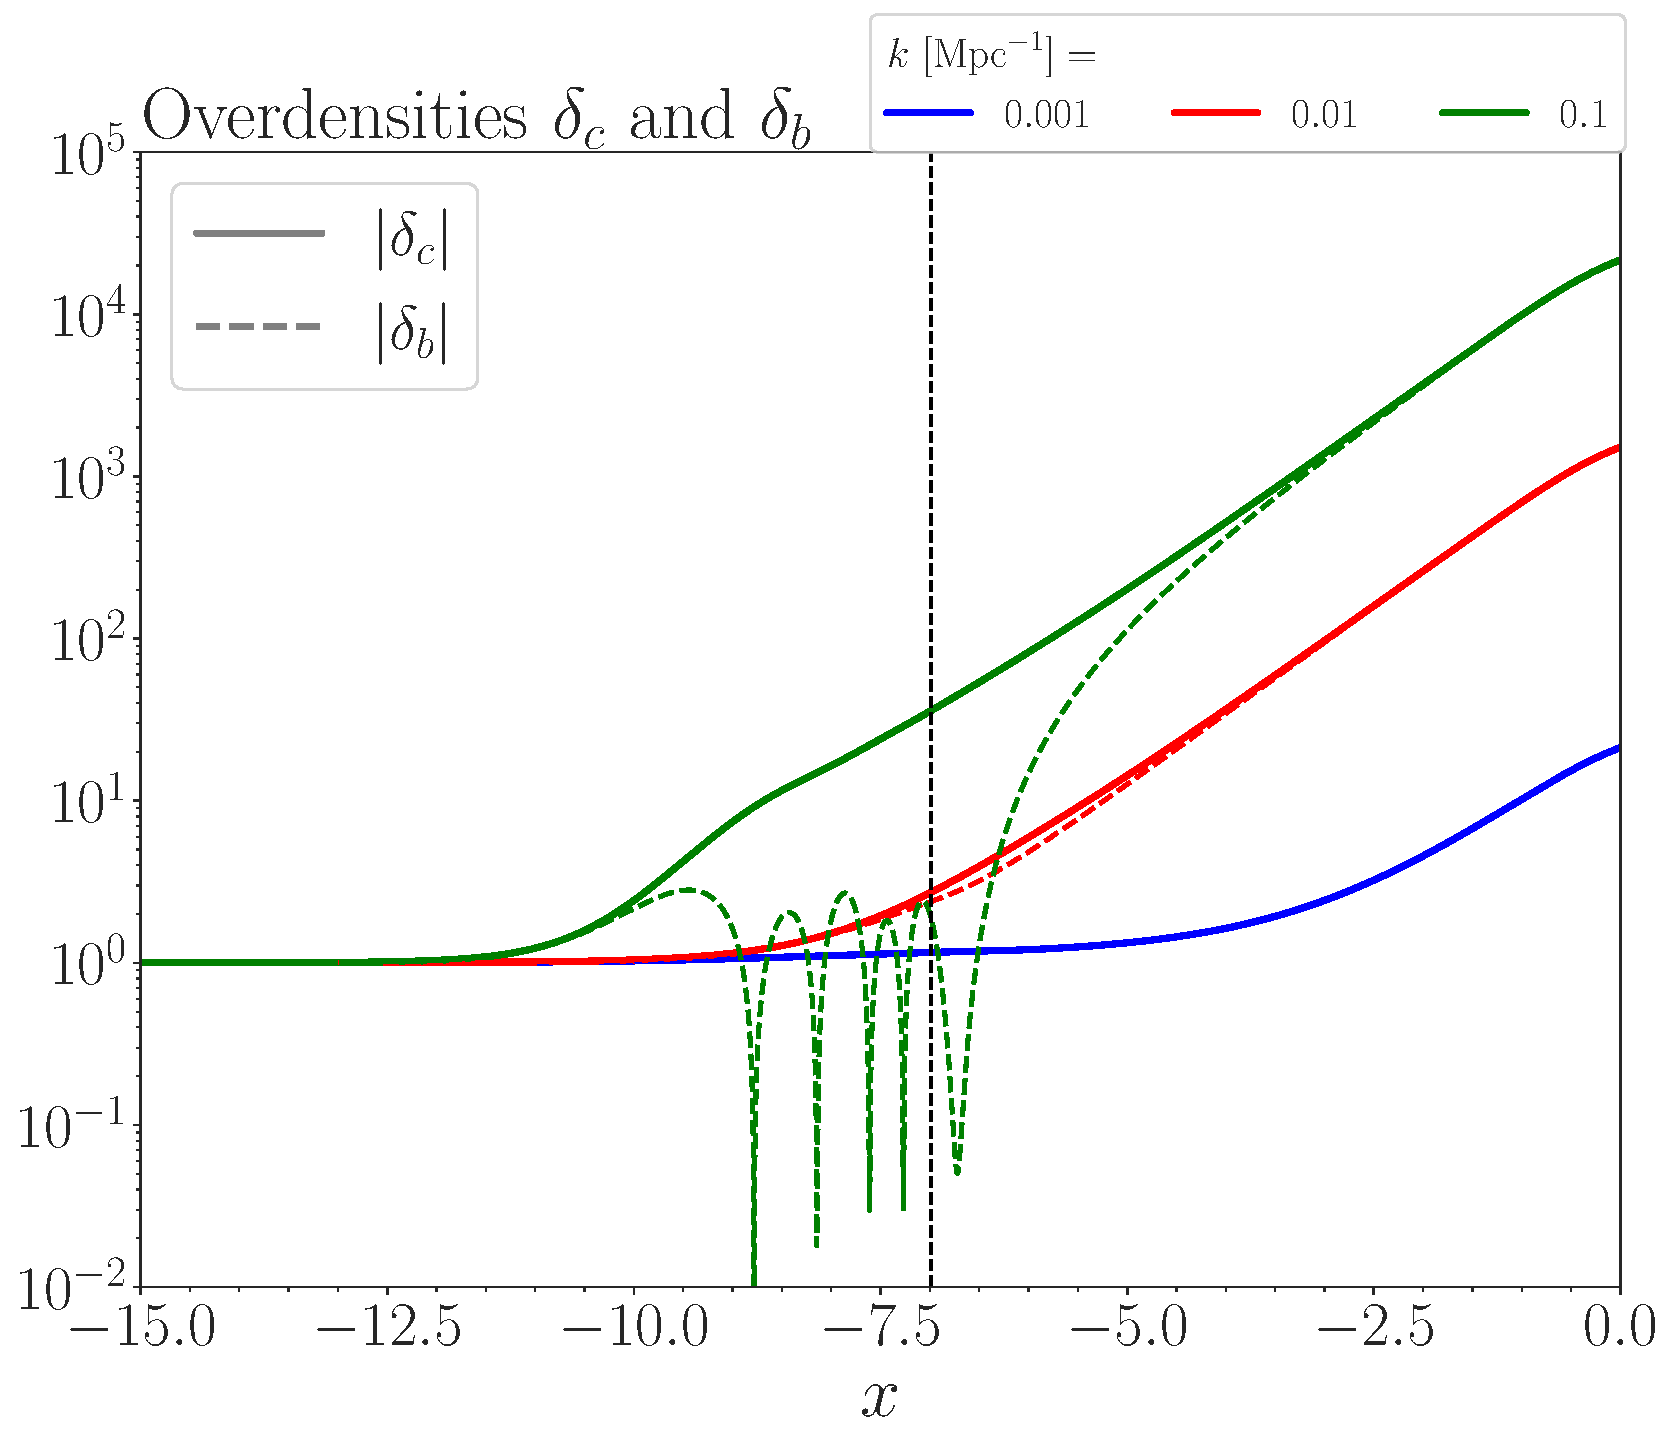
\includegraphics[width=\linewidth]{delta.pdf}
        \caption{delta term}
        \label{fig:m3:delta}
    \end{figure}

    \begin{figure}
        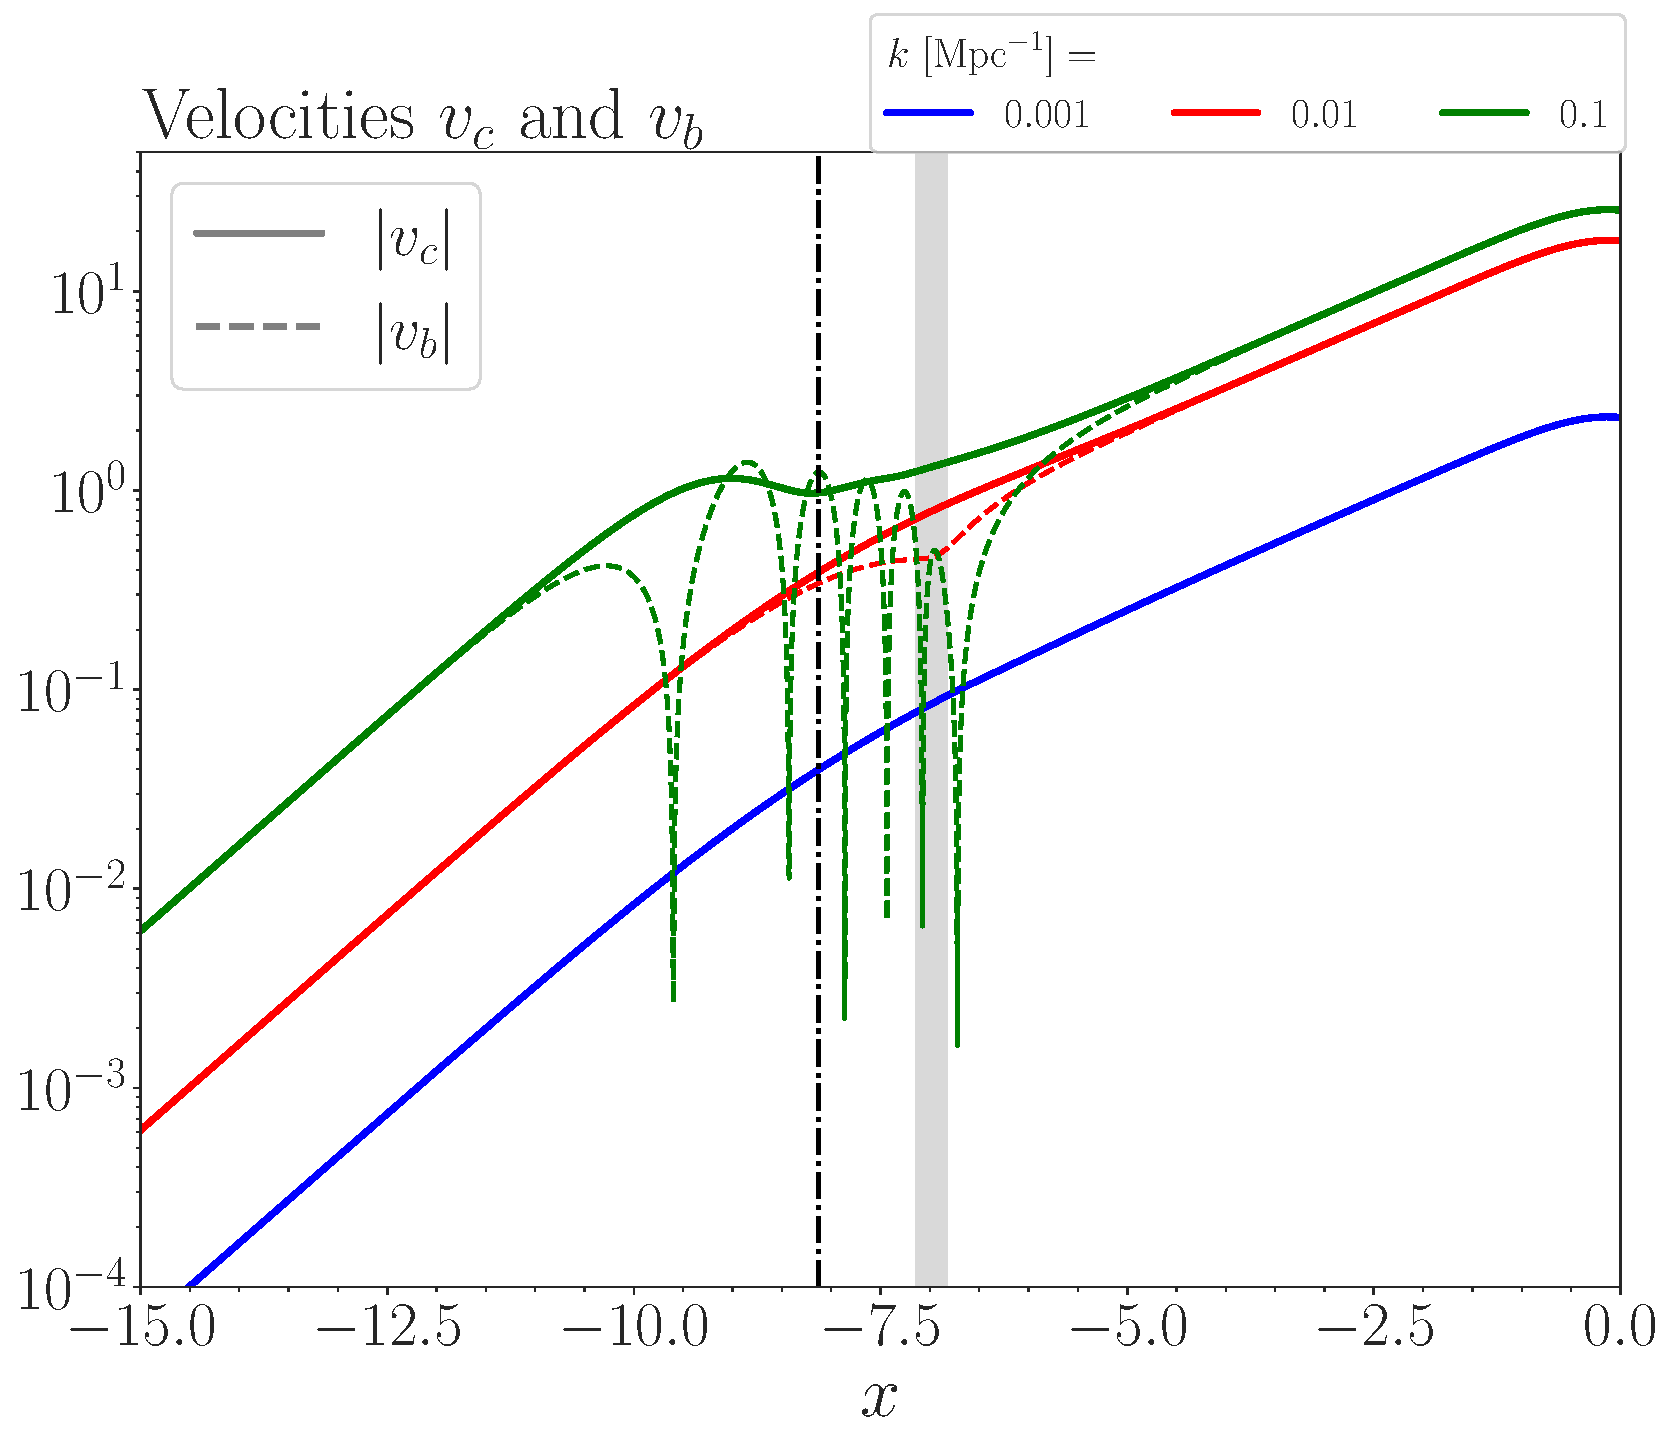
\includegraphics[width=\linewidth]{velocity.pdf}
        \caption{Velocities term}
        \label{fig:m3:velocity}
    \end{figure}

    \begin{figure}
        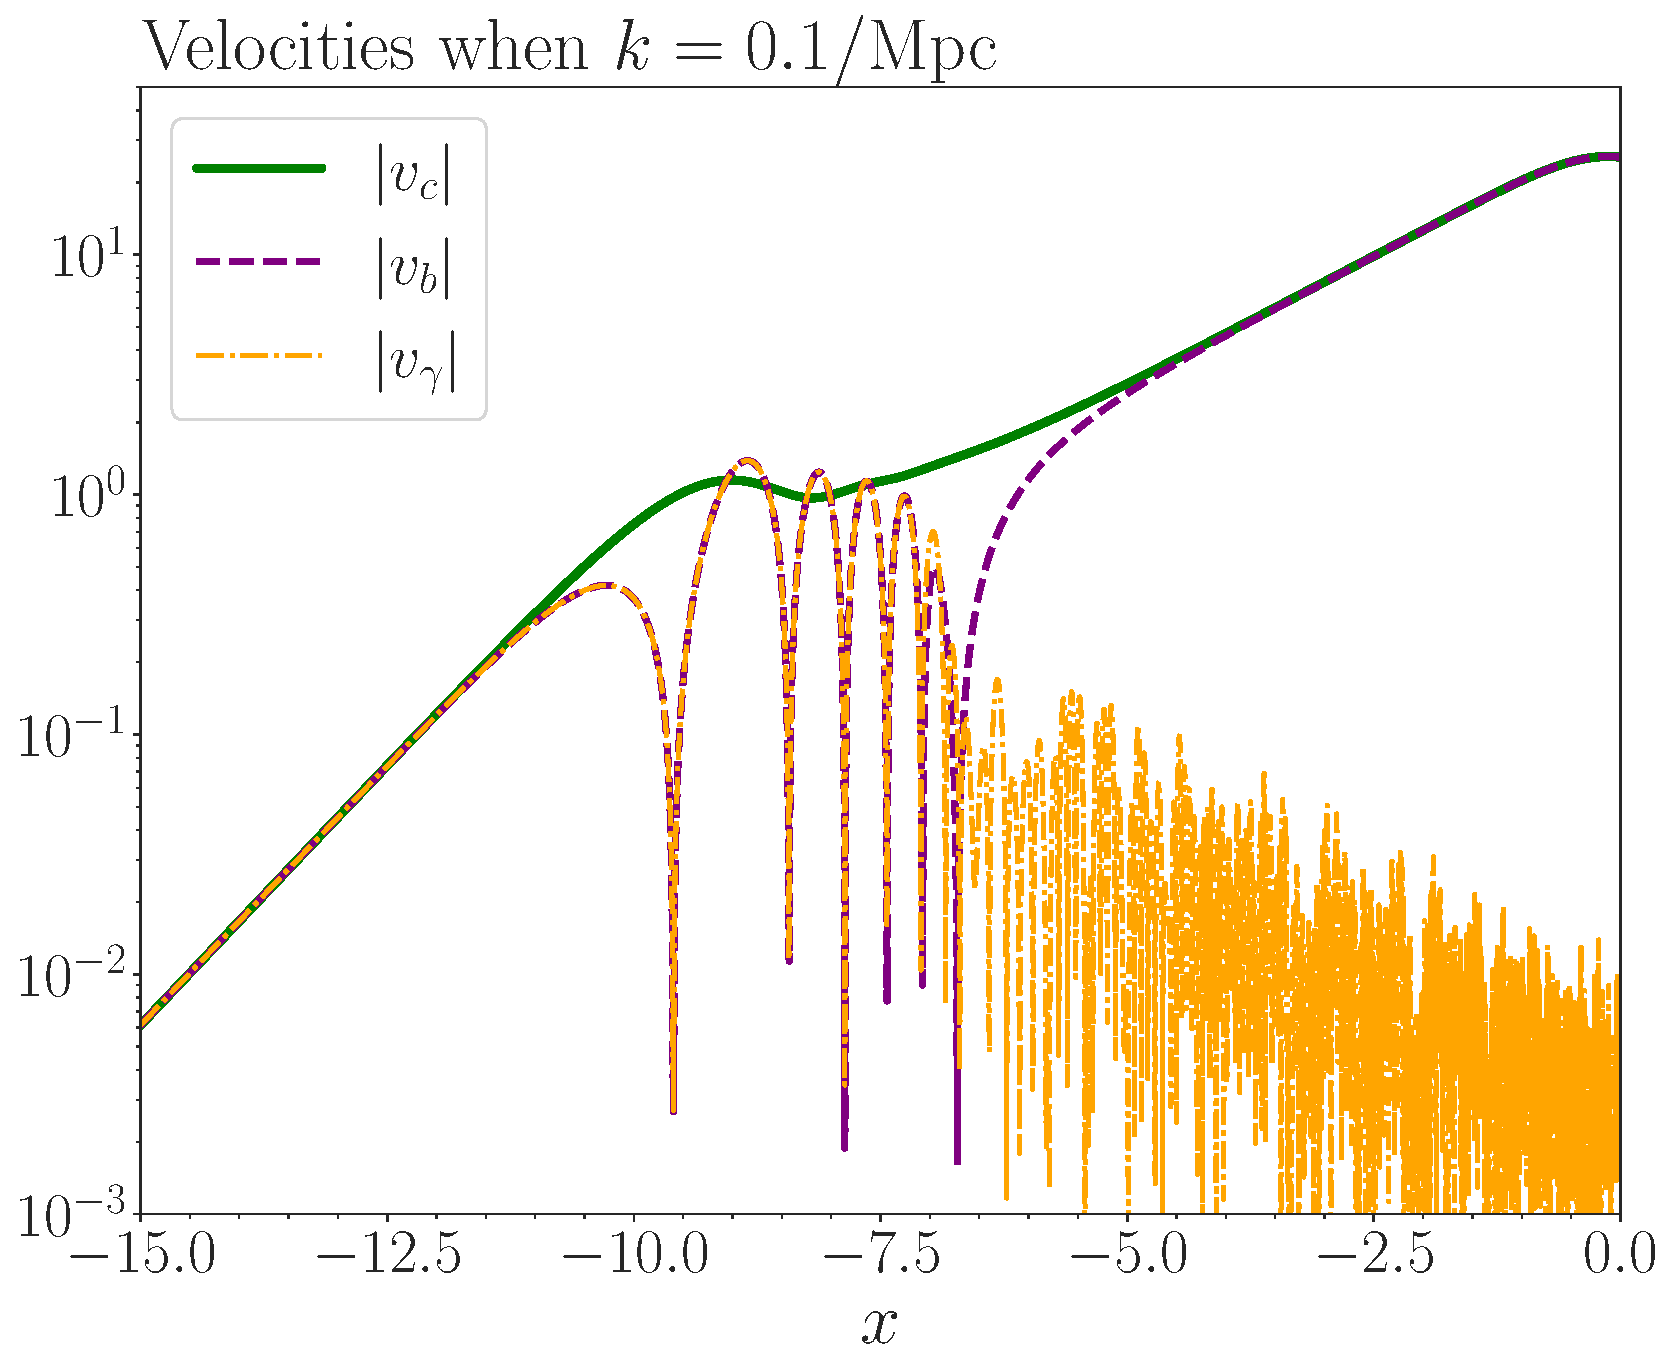
\includegraphics[width=\linewidth]{velocity_comparison.pdf}
        \caption{Velocities term}
        \label{fig:m3:velocity_comparison}
    \end{figure}

    \begin{figure}
        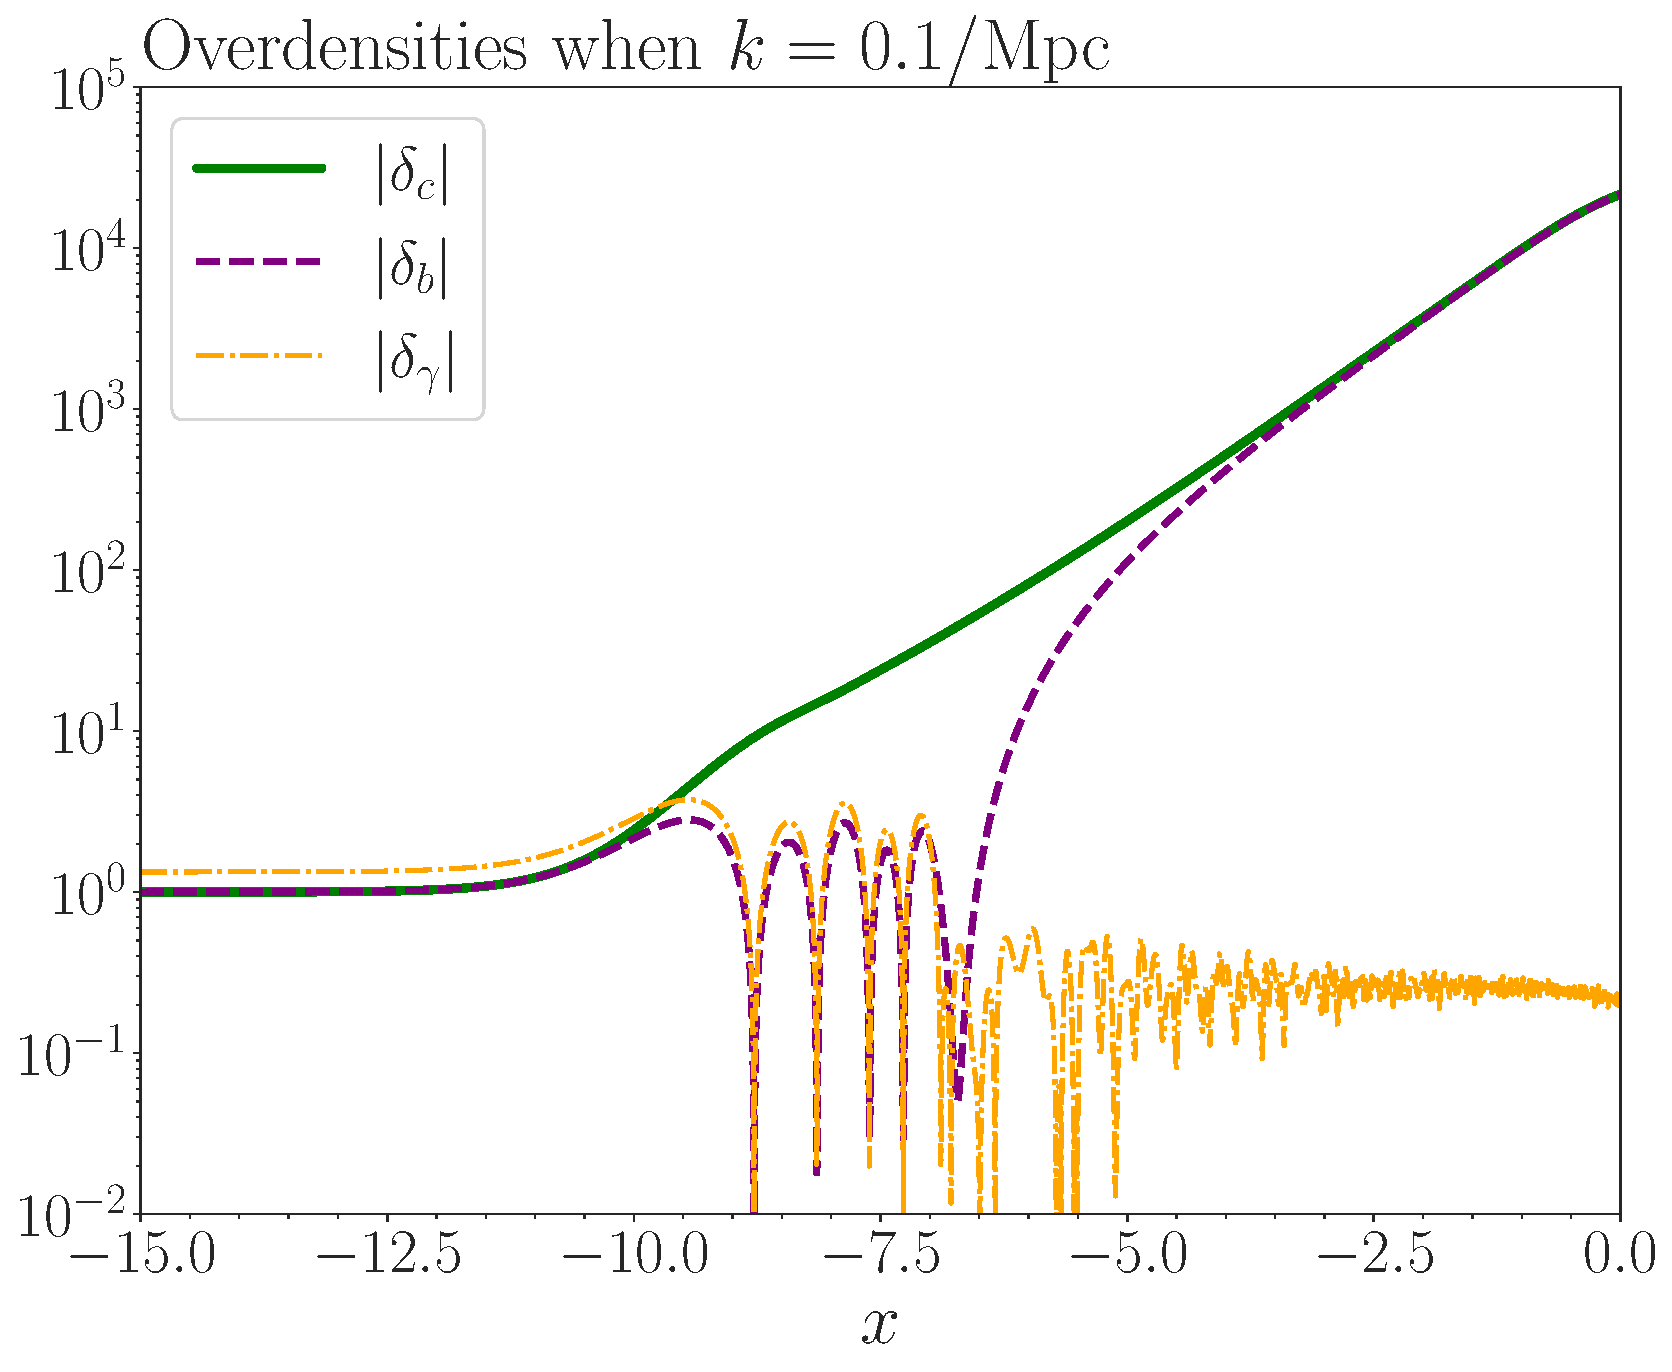
\includegraphics[width=\linewidth]{delta_comparison.pdf}
        \caption{Velocities term}
        \label{fig:m3:delta_comparison}
    \end{figure}

